\documentclass[border=0.125cm]{standalone}
\usepackage{tikz}
\usepackage[T1]{fontenc}
\usepackage{newtxtext, newtxmath}
\usetikzlibrary{positioning}
\begin{document}

\tikzset{%
  every neuron/.style={
      circle,
      draw,
      minimum size=1cm
    },
  neuron missing/.style={
      draw=none,
      scale=4,
      text height=0.333cm,
      execute at begin node=\color{black}$\vdots$
    },
}

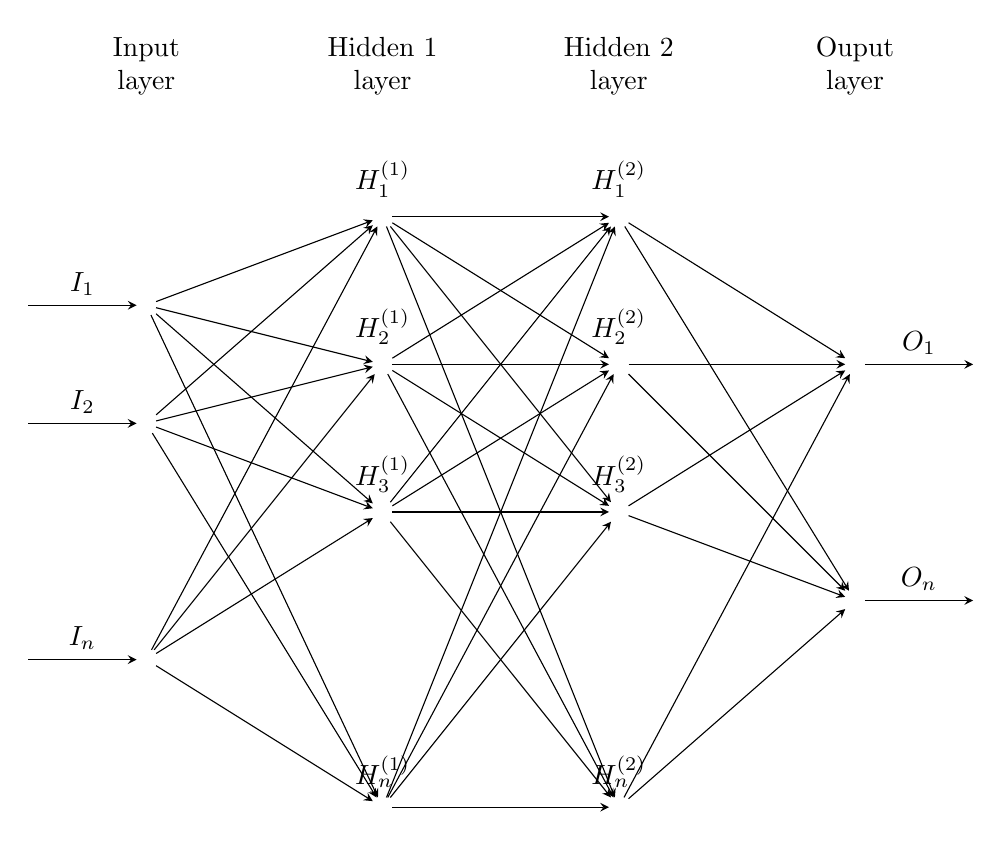
\begin{tikzpicture}[x=1.5cm, y=1.5cm, >=stealth]

  \foreach \m/\l [count=\y] in {1,2,missing,3}
  \node [every neuron/.try, neuron \m/.try] (input-\m) at (0,2.0-\y) {};

  \foreach \m [count=\y] in {1,2,3,missing,4}
  \node [every neuron/.try, neuron \m/.try ] (hidden1-\m) at (2,3-\y*1.25) {};

  \foreach \m [count=\y] in {1,2,3,missing,4}
  \node [every neuron/.try, neuron \m/.try ] (hidden2-\m) at (4,3-\y*1.25) {};

  \foreach \m [count=\y] in {1,missing,2}
  \node [every neuron/.try, neuron \m/.try ] (output-\m) at (6,1.5-\y) {};

  \foreach \l [count=\i] in {1,2,n}
  \draw [<-] (input-\i) -- ++(-1,0)
  node [above, midway] {$I_\l$};

  \foreach \l [count=\i] in {1,2,3,n}
  \node [above] at (hidden1-\i.north) {$H^{(1)}_\l$};

  \foreach \l [count=\i] in {1,2,3,n}
  \node [above] at (hidden2-\i.north) {$H^{(2)}_\l$};

  \foreach \l [count=\i] in {1,n}
  \draw [->] (output-\i) -- ++(1,0)
  node [above, midway] {$O_\l$};

  \foreach \i in {1,...,3}
  \foreach \j in {1,...,4}
  \draw [->] (input-\i) -- (hidden1-\j);

  \foreach \i in {1,...,4}
  \foreach \j in {1,...,4}
  \draw [->] (hidden1-\i) -- (hidden2-\j);

  \foreach \i in {1,...,4}
  \foreach \j in {1,...,2}
  \draw [->] (hidden2-\i) -- (output-\j);

  \foreach \l [count=\x from 0] in {Input, Hidden 1, Hidden 2, Ouput}
  \node [align=center, above] at (\x*2,2.7) {\l \\ layer};

\end{tikzpicture}

\end{document}